\documentclass[letterpaper,12pt,twoside]{book}  % book class
%\usepackage[spanish,es-nodecimaldot,es-tabla]{babel} % language/hyphenation
\usepackage[english]{babel}
\usepackage[utf8]{inputenc}  % input encoding
\usepackage{graphicx} % graphics library (REQUIRED by CIMATpreamble)
\usepackage[svgnames,table]{xcolor}  % color library (REQUIRED by CIMATpreamble)
\usepackage{CIMATpreamble}  % definition of the CIMAT cover page
\usepackage{mypreamble} % custom preamble
\graphicspath{{img/}}  % set path for images folder

%-----------------------------------------------------------------------------%
% Coverpage template requested by CIMAT for the master thesis in LaTeX version 

%-----------------------------------------------------------------------------%
% README: Instructions & Comments
%
% > The package 'CIMATpreamble' is required for the CIMAT cover page and 
%   it depends on the declared libraries above
% > To use the COVER template only fill the Cover/Titlepage block 
%   with your information and make sure the '\maketitle' command is enabled
%
% > The rest of the LaTeX code was built according to the guideline provided by 
%   the ShareLatex/Overleaf team:
%   "How to Write a Thesis in LaTeX (Part 1): Basic Structure"; you will find  
%   the custom settings (link colors, caption specs., etc.) in the 
%   'mypreamble.sty' file, so you are free to use or modify that code 
% > Much of the code for the cover page is based on the Overleaf template    
%   created by Salvador Pedraza Espitia: 
%   https://www.overleaf.com/latex/templates/unam-dissert/mypjkyrmhgns
% > The essential idea of this code is to provide a minimal and functional  
%   LaTeX document, allowing us to focus on the content of our thesis work;
%   I hope it be useful for you :) !
% 
% > Credits: Kenny Yahir Mendez Ramirez, Cristal E. Mendez Ramirez
% > For comments and suggestions please send a e-mail to kenny.yahir.mz@gmail.com

%-----------------------------------------------------------------------------%
% Cover/Title page: fill out with your personal information

\author{Ivonne Monter Aldana}
\documentType{T E S I S}  % change to "T E S I N A" if it is the case
\title{Transformers\ldots}
\degree{Maestra en Ciencias con especialidad en Computación y Matemáticas Industriales}
\supervisor{Dr.Adrián Pastor López Monroy}
\supervisorSecond{}  % optional command
\cityandyear{Guanajuato, Gto, Noviembre de 2021}


%-----------------------------------------------------------------------------%
% Document body

\begin{document}

% Coverpage
\maketitle  % this enable the CIMAT title page!

\thispagestyle{empty}  % blank page after title page

\frontmatter

% Dedication
\chapter*{}
\begin{flushright}%
  \emph{Dedicatoria \ldots}
  \thispagestyle{empty}
\end{flushright}

% Abstract
\chapter*{Abstract}
\addcontentsline{toc}{chapter}{Abstract}


\\
% Keywords
\paragraph{Keywords:} 

% Acknowledgements
\chapter*{Acknowledgments}
\addcontentsline{toc}{chapter}{Acknowledgments}

A mis padres \ldots

% Table of contents and list of figures
\tableofcontents

\listoffigures

% Chapters
\mainmatter

\spacing{1.5}  % interline  (double) space

% put the content of your chapters in the .tex files located in the 'chapters/' folder; 
% the use of '\include' instead of '\input' command could enhance the  compilation process, see the reference below

\chapter{Introducction}

 \ldots


\section{Related work} \label{sec:problem}


\section{Our Goals}

%\section{Contribution} \label{sec:contribution}



\section{Thesis Overview}








\chapter{Background} \label{chap:background}
\section{Text Classification}
\subsection{Transformers}
\section{Image Classification}
\subsection{Transformers on image}
\section{Multimodal Classification}
\subsection{Metrics}

\chapter{Análisis Exploratorio}\label{chap:eda}

\section{Bases de datos}


\begin{figure}[H]
\centering
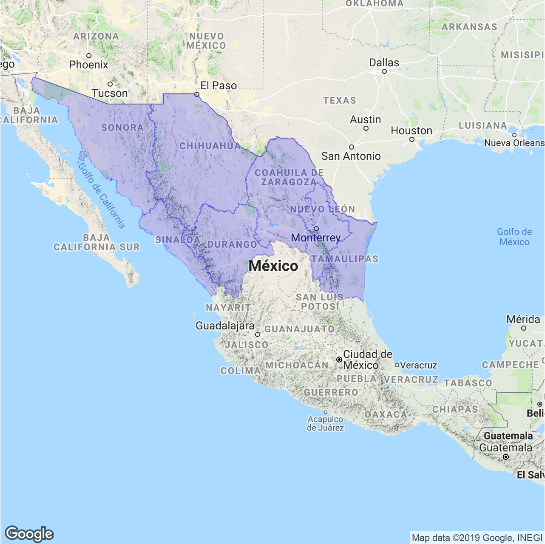
\includegraphics[width = 11cm]{ggmap_7_entidades_sample_02}  % using \graphicspath specification
\caption{Selección de 7 estados de la República Mexicana para la modelación. Este mapa fue construido con el uso de \texttt{ggmap} \citep{Kahle2013ggmap} y requirió la activación de los servicios de Google Maps.}
\label{fig:selecc_entidades_01}
\end{figure}

\chapter{Modelación espacio-temporal} \label{chap:modeling}

\section{Modelos espaciales} \label{sec:spatial_models}

\subsubsection{Modelo Poisson-Gamma} \label{subsubsec:bayesian_poisson_gamma}

Para este tipo de modelos es posible utilizar representaciones gráficas que reflejen la estructura de dependencias en la jerarquía. Esta representación es conocida como \textit{Grafo Acíclico Dirigido} (DAG). Las aristas conectan los niveles de la jerarquía y los parámetros son los vértices al final de las aristas (flechas). Es importante establecer un límite en la jerarquía ya que no es posible asumir una jerarquía de parámetros infinita. Usualmente el punto de corte se elige donde la variación de los hiperparámetros ya no afecta al nivel más bajo del modelo (primer nivel). En este punto los parámetros se asumen como valores fijos. Por ejemplo en el modelo \textit{Poisson-Gamma} si se fijan $\alpha$ y $\beta$ entonces la distribución a priori \textit{Gamma} será fija y los datos no nos darán información acerca de la distribución en lo absoluto. Sin embargo podemos permitir un nivel mayor de variación asignando hiperdistribuciones a priori para $\alpha$ y $\beta$, fijando los valores de $\nu$ y $\rho$ sin afectar radicalmente el nivel más bajo de variación. La \autoref{fig:dag_poisson_gamma} muestra el DAG para el modelo \textit{Poisson-Gamma} de dos niveles \citep{lawson2013bayesian}.

\begin{figure}[htb!]
\centering
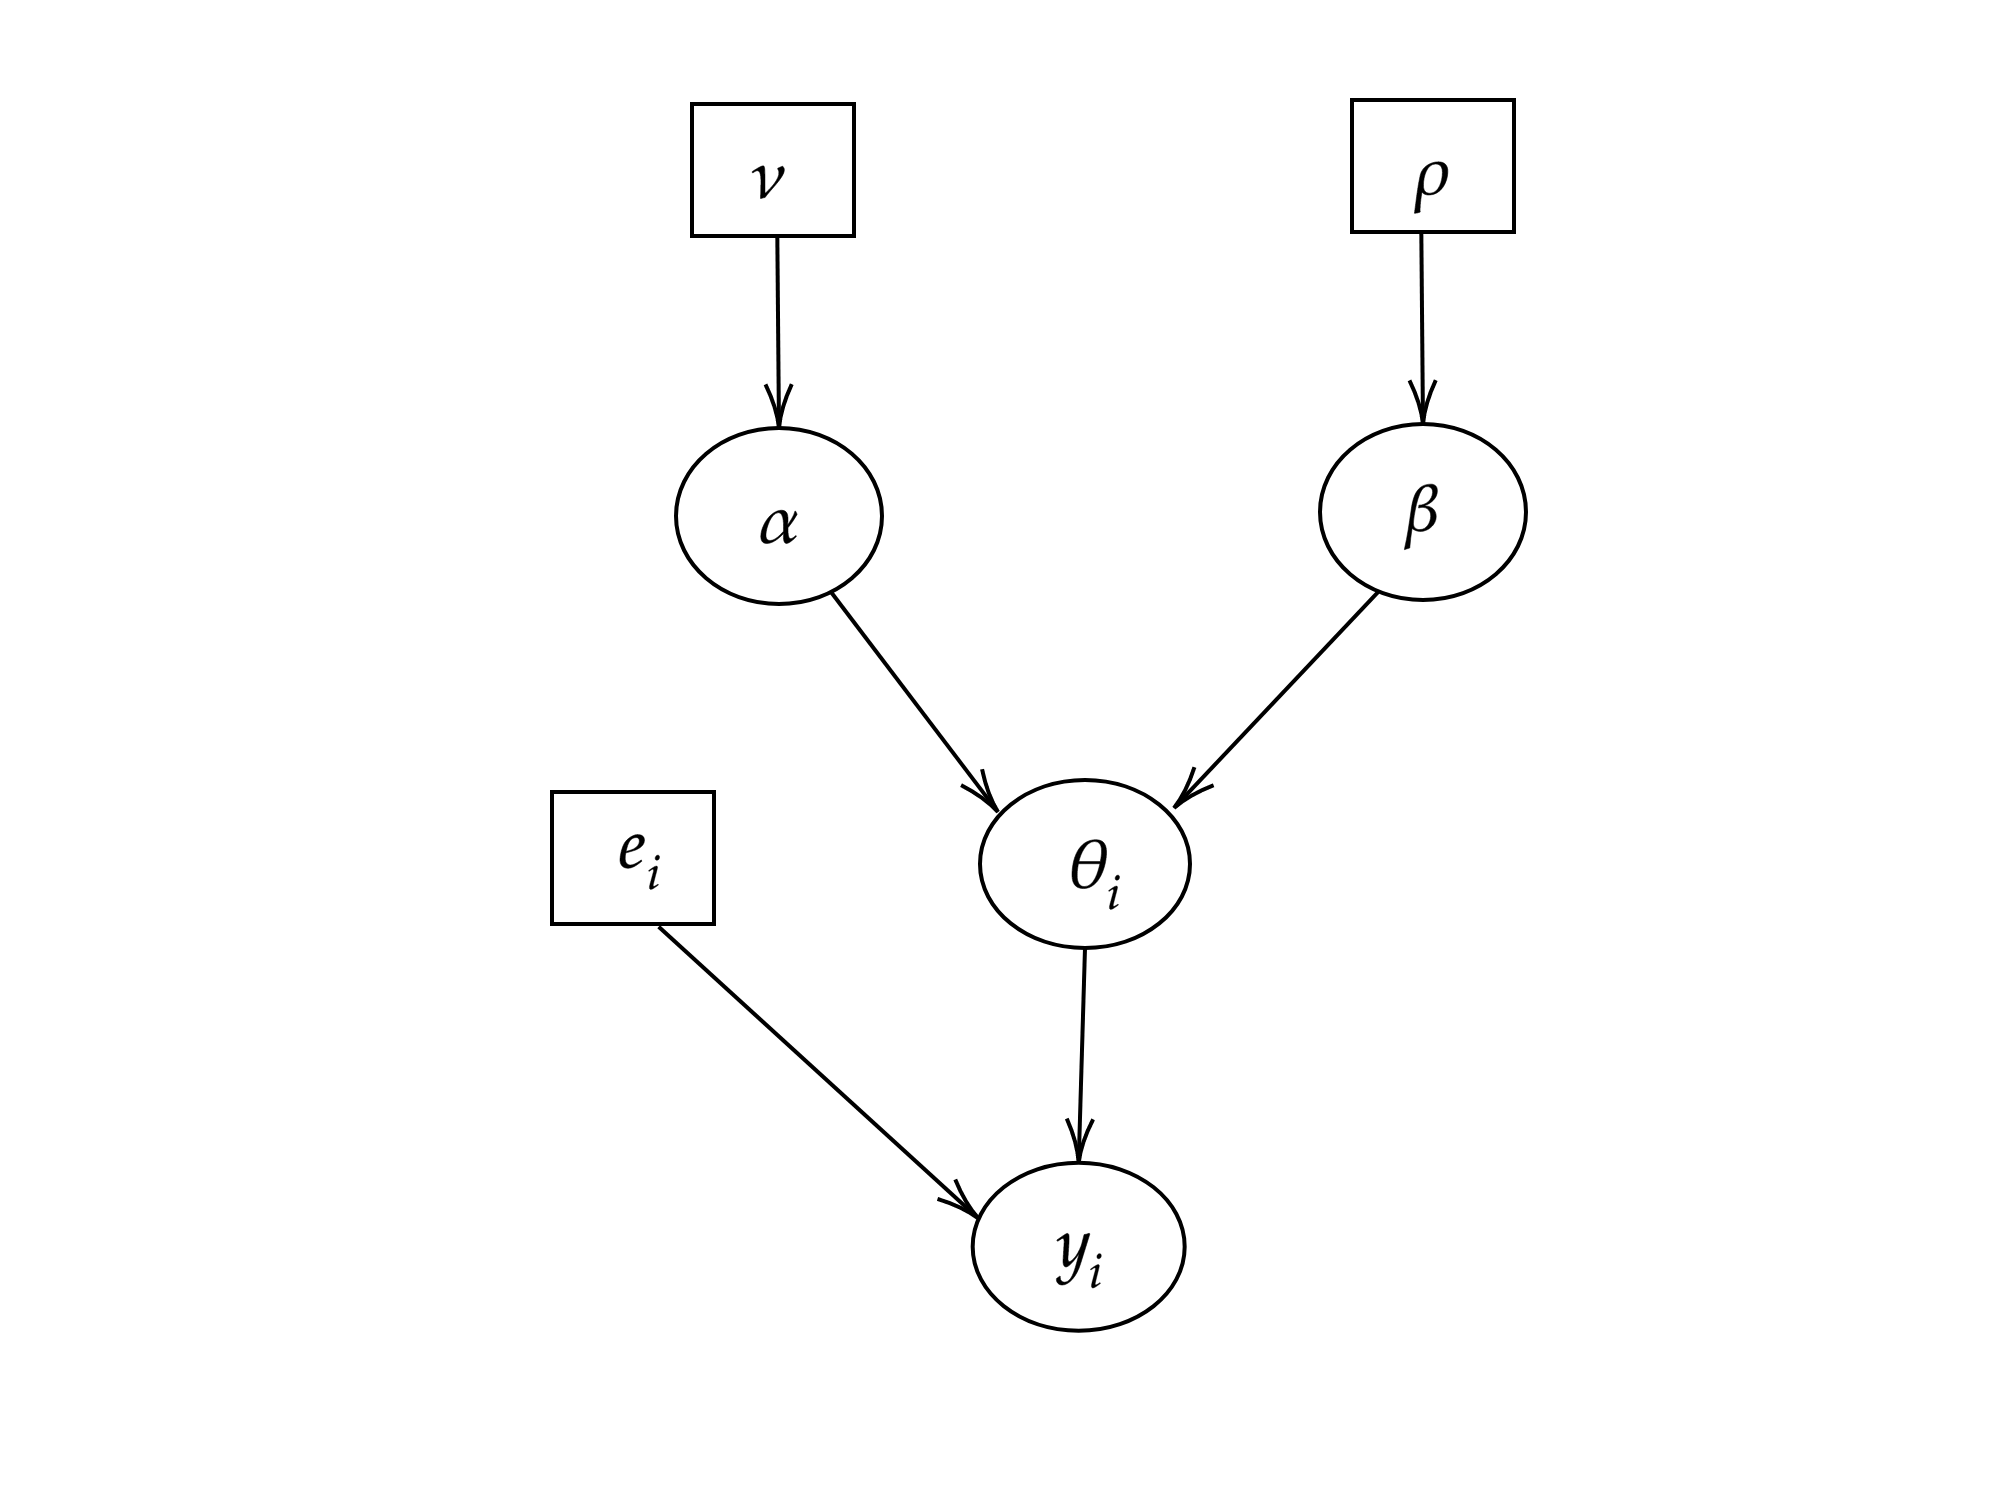
\includegraphics[width=0.8\textwidth]{img/example_hbm_lawson_01}
\caption{Gráfica Acíclica Dirigida de la representación jerárquica del modelo Poisson-Gamma.}\label{fig:dag_poisson_gamma}
\end{figure}

\chapter{Conclusiones y trabajo futuro}

% Bibliography
\bibliographystyle{apacite}  % APA style according to apacite package: see mypreamble.sty line 21
\bibliography{references}

% Appendix
\appendix
\chapter{Anexo}

\backmatter

\end{document}

% LaTeX references (technical issues, workarounds)

% https://www.overleaf.com/learn/latex/Management_in_a_large_project ('including files' section)
% https://tex.stackexchange.com/questions/64839/how-to-change-listing-caption
% https://stackoverflow.com/questions/2709898/change-list-of-listings-text
% https://tex.stackexchange.com/questions/664/why-should-i-use-usepackaget1fontenc